\section{Tower}
\subsection*{题意}
给 $n$ 块砖,第 $i$ 块砖的重量为 $w_i$,坚硬度为 $s_i$,权值为 $v_i$。

现在需要选取若干块砖自下而上垒成一座塔,每层恰好有一块砖。对于每一块砖,它上面所有砖的重量之和不能超过他的坚硬度。

求最大化的选取的砖的权值之和。
\subsection*{数据范围}
\begin{itemize}
\item $1 \leq n \leq 10^3$
\item $1 \leq w_i, s_i \leq 10^4$
\item $1 \leq v_i \leq 10^9$
\end{itemize}

\subsection*{题解}

这题的难点我们既要选取子集还要规定一个顺序,所以我们先思考如何在给定顺序下选取最优子集。


首先注意到这样的事实:在最上层垒一块砖相当于把之前的每一块砖的坚硬度同时减去当前砖的重量,所以根据木桶原理,我们只需要关心最脆弱的砖,而不需要关心每块砖各自的承重。

假设之前最大承重为 $j$,当前砖的重量为 $w$,坚硬度为 $s$,那么在把当前砖垒上去之后新的最大承重为 $\min(j-w,s)$。

现在规定排在后面的砖只能在垒在前面的上方,我们设 $\texttt{dp}[i][j]$ 表示前 $i$ 块砖最多还能承受的重量是 $j$ 的最大权值。和背包的思想类似,容易得到转移:
\begin{align*}
    \texttt{dp}[i+1][j] &\longleftarrow \texttt{dp}[i][j] &\text{不选} \\
    \texttt{dp}[i+1][\min(j-w_{i+1},s_{i+1})] &\longleftarrow \texttt{dp}[i][j] + v_{i+1}&\text{选}\\
\end{align*}

初始条件为 $\texttt{dp}[0][\infty] = 0$。

\newpage
\begin{center}
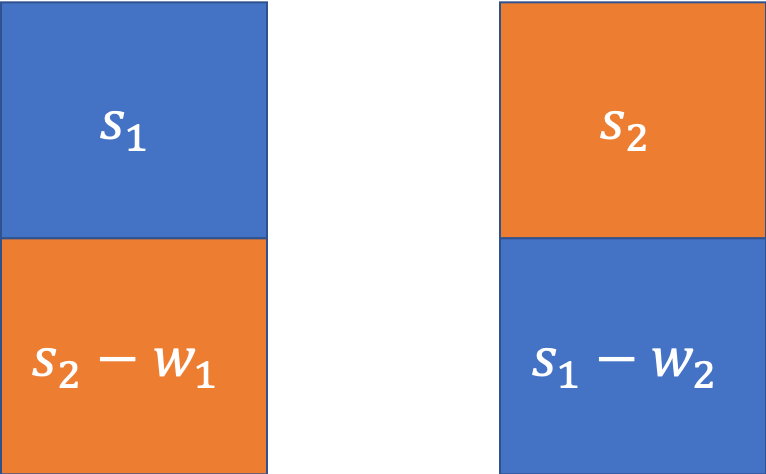
\includegraphics[width=5cm]{./Pics/tower.png}
\end{center}
\paragraph{确定顺序} 现在我们考虑如何确定添加的顺序。

假设最优解中有相邻的两块砖 $1$和 $2$,坚硬度为 $s_1,s_2$,重量为 $w_1,w_2$。左图中 $1$ 在上方,右图中 $2$在上方。 

两种方式得到的最大承重分别是 $\min(s_1,s_2-w_1)$ 和 $\min(s_2,s_1-w_2)$。由于两种方式对于权值的贡献都是 $v_1+v_2$,我们只需要选择能最大化承重的那种即可。

假设 $s_2-w_1\ge s_1-w_2$。由于 $s_1$ 显然大于 $s_1 - w_2$,所以可以得到:
$$
\min(s_1,s_2-w_1) \ge s_1-w_2 \ge \min(s_2,s_1-w_2)
$$

所以在 $s_2-w_1\ge s_1-w_2$ 的情况下,把 $2$ 放在下面肯定是更好的选择(至少不会更差)。注意到这个条件等价于  $s_2 +w_2 \ge s_1+w_1$,所以我们可以把所有砖按照 $s_i + w_i$ 从大到小排序,以这个顺序垒起来的砖块一定是最优的。



\subsection*{核心代码}
\inputminted[linenos,autogobble]{cpp}{./Code/X.cpp}
\newpage